\appendix

\chapter{Vollständiger Aufbau des LSS-Formates}
\label{app:lss}

\begin{figure}[h]
			\centering
			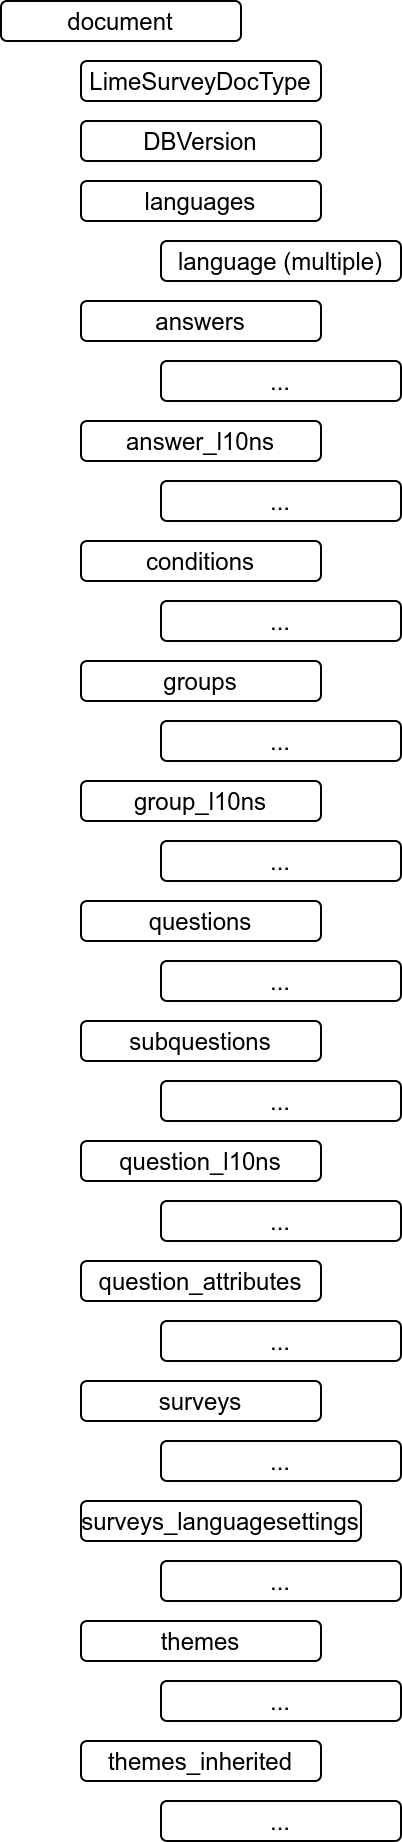
\includegraphics[width=.25\textwidth]{./img/append_lss.png}
			\caption{Aufbau des Wurzel-Elements \el{document}}
			\label{app:lss_struct}
\end{figure}

\begin{figure}[h]
	\centering
	\begin{subfigure}[b]{.45\textwidth}
		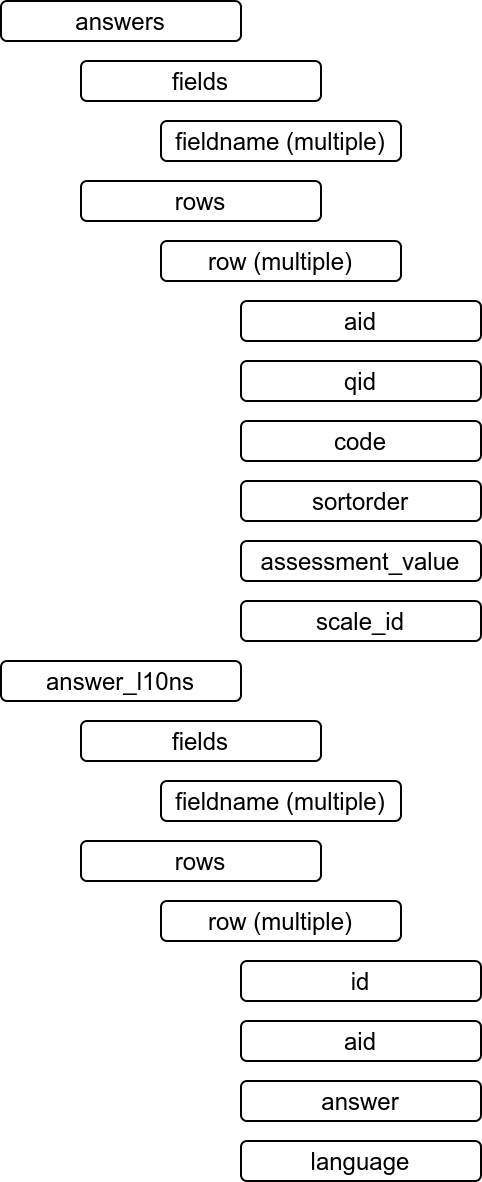
\includegraphics[width=.95\textwidth]{./img/append_lss_ans.png}
		\caption{Aufbau der Elemente für die Antworten}
	\end{subfigure}%
	\begin{minipage}[b]{.45\textwidth}
		\begin{subfigure}[b]{\linewidth}
			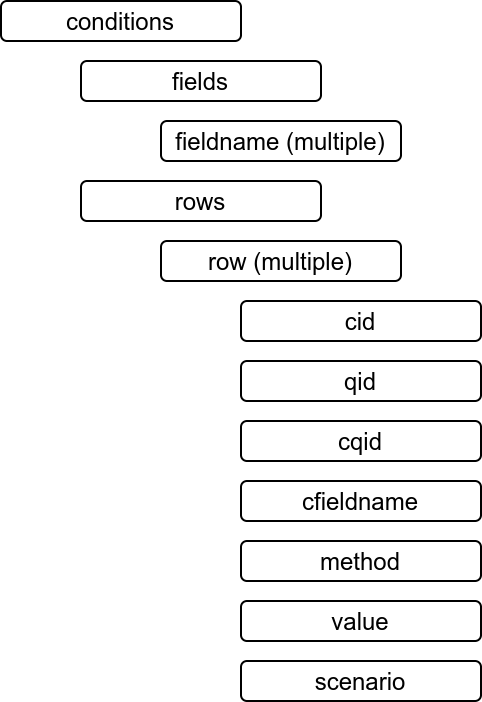
\includegraphics[width=.95\textwidth]{./img/append_lss_cond.png}
			\caption{Das Element für die Bedingungen}
		\end{subfigure}\\
		\begin{subfigure}[b]{\linewidth}
			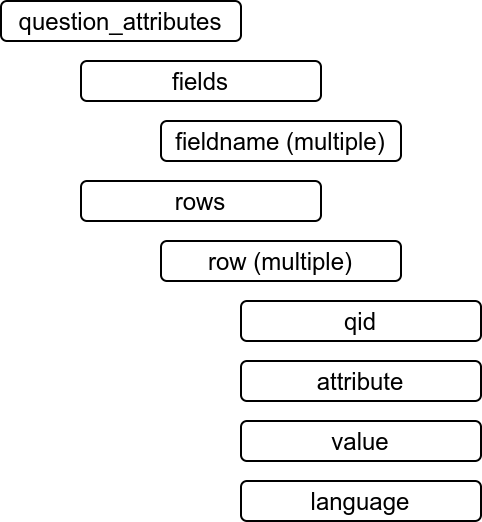
\includegraphics[width=.95\textwidth]{./img/append_lss_q_attr.png}
			\caption{Die Frageattribute im LSS-Format}
		\end{subfigure}%
	\end{minipage}
\end{figure}

\begin{figure}[h]
	\makebox[\linewidth][c]{%
		\begin{subfigure}[b]{.45\textwidth}
			\centering
			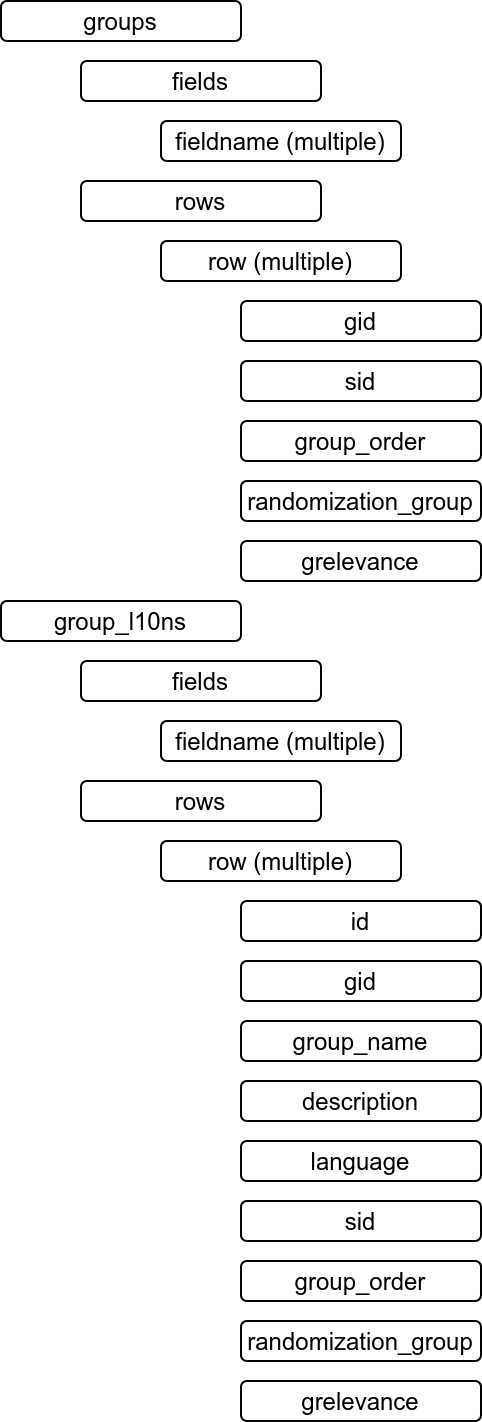
\includegraphics[width=.95\textwidth]{./img/append_lss_group.png}
			\caption{Aufbau von Fragegruppen}
		\end{subfigure}%
		\begin{subfigure}[b]{.45\textwidth}
			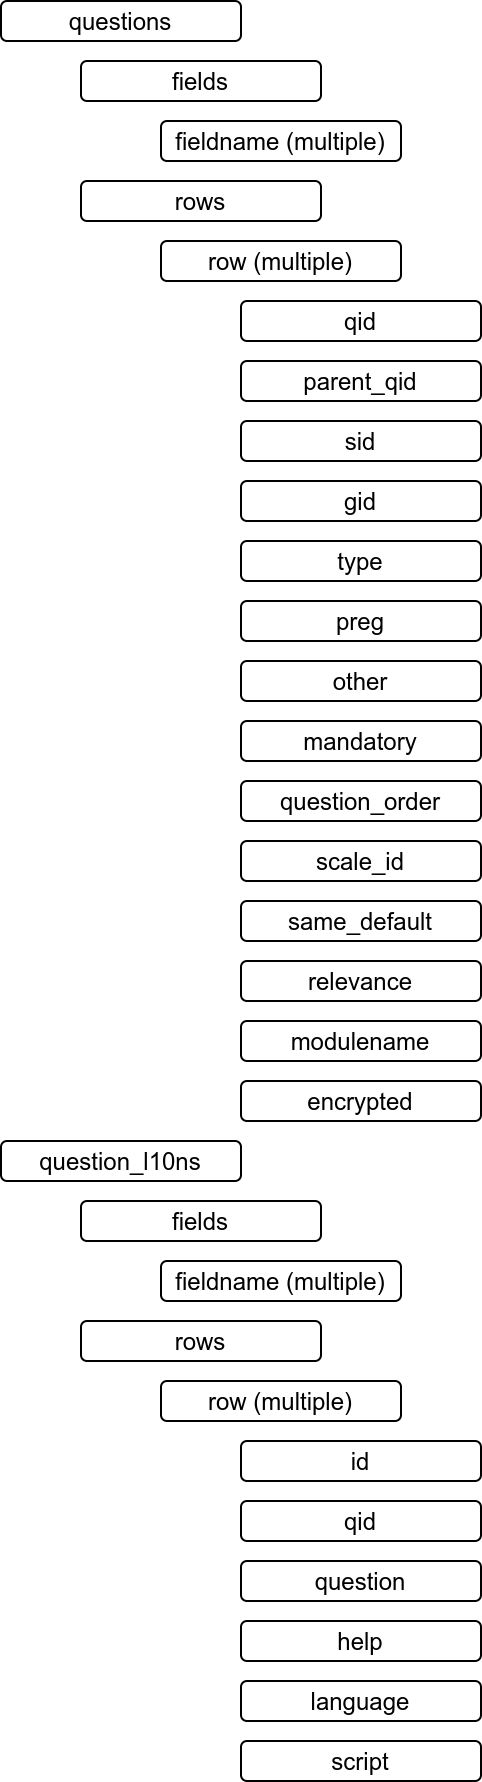
\includegraphics[width=.95\textwidth]{./img/append_lss_q.png}
			\caption{Aufbau der Frageelemente}
		\end{subfigure}%
		}
		\caption{Diagramme für Fragegruppen und Fragen}
\end{figure}

\begin{figure}[h]
	\centering
	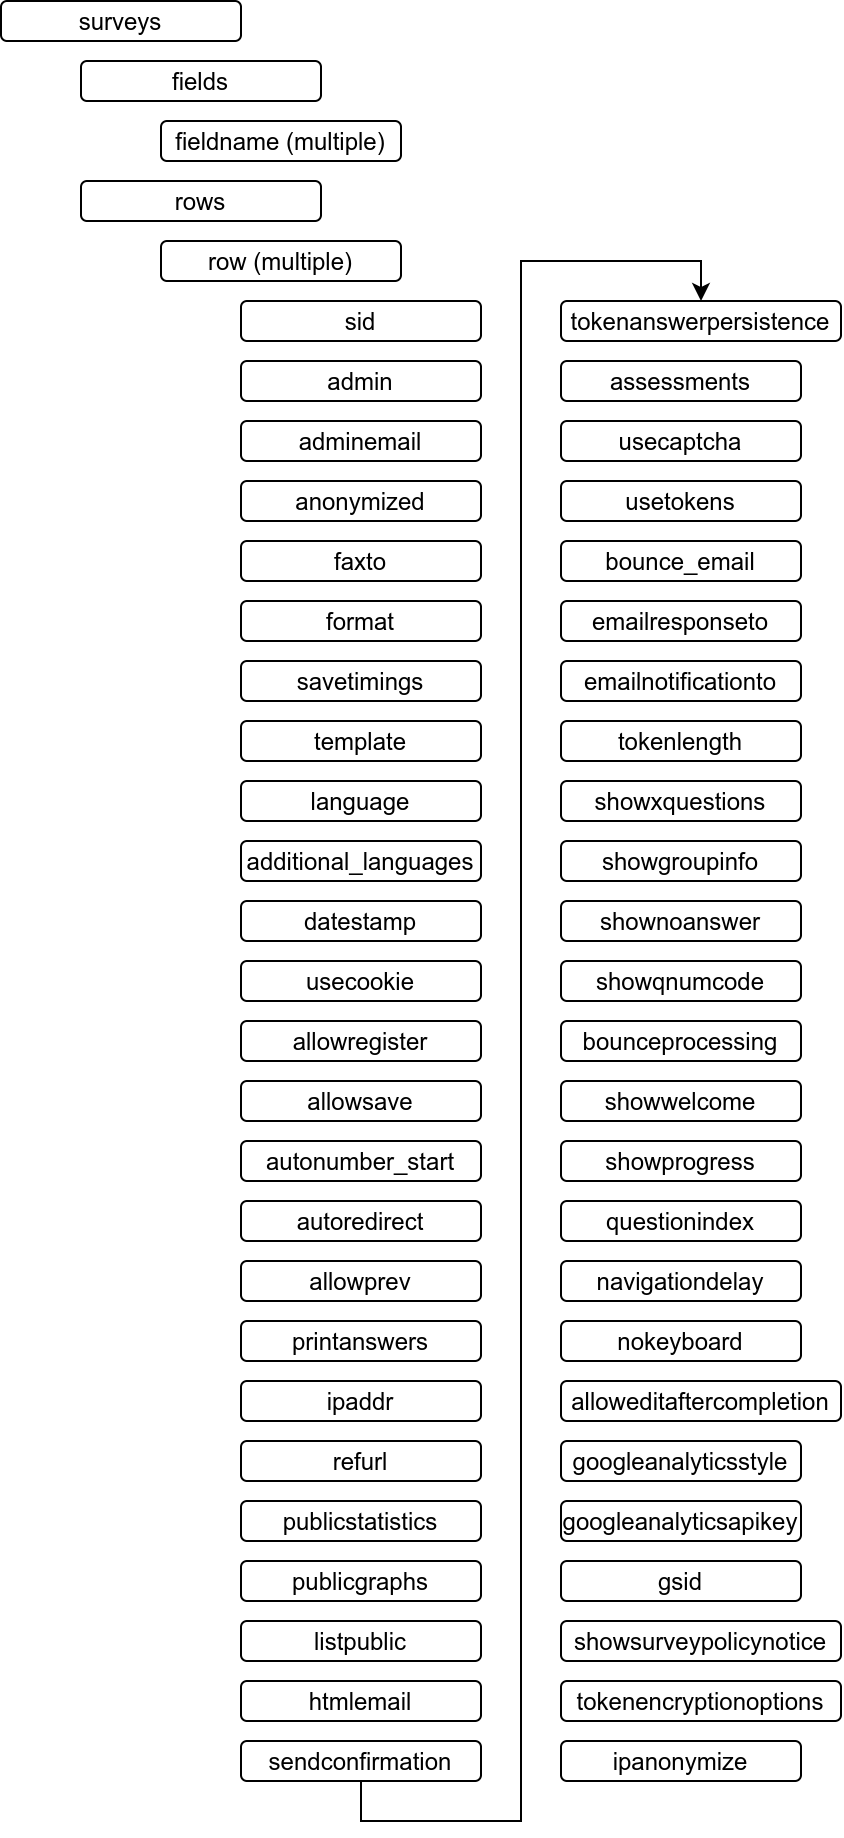
\includegraphics[width=.7\textwidth]{./img/append_lss_sur.png}
	\caption{Aufbau der Metadaten einer Umfrage}
\end{figure}

\begin{figure}[h]
	\makebox[\linewidth][c]{%
		\begin{subfigure}[b]{.45\textwidth}
			\centering
			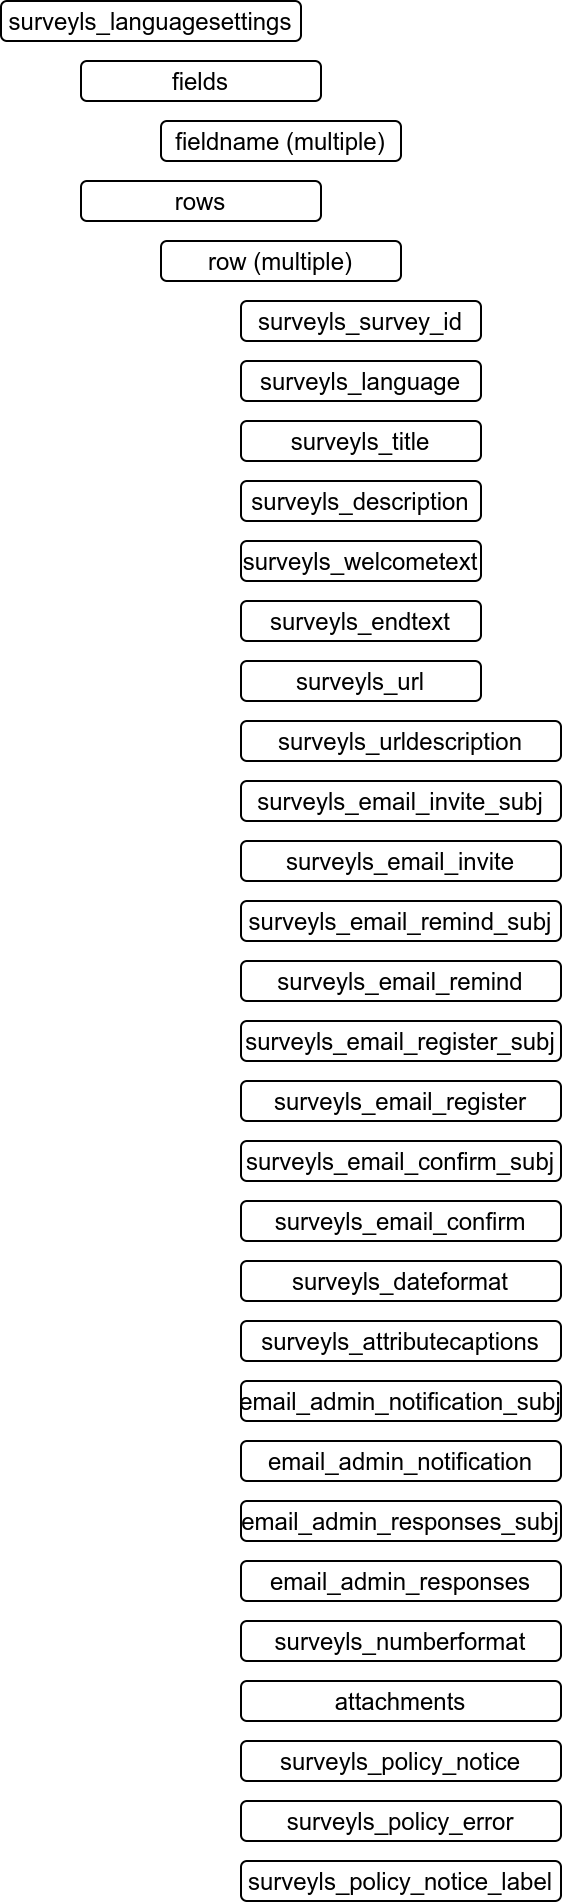
\includegraphics[width=.95\textwidth]{./img/append_lss_surls.png}
			\caption{Aufbau von weiteren Metadaten der Umfrage}
		\end{subfigure}%
		\begin{subfigure}[b]{.45\textwidth}
			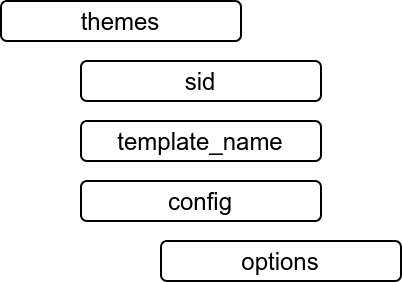
\includegraphics[width=.8\textwidth]{./img/append_lss_theme.png}
			\caption{Aufbau eines Themes}
		\end{subfigure}%
		}
		\caption{Diagramme für Metadaten der Umfrage und des Designs}
\end{figure}

\begin{figure}[h]
	\centering
	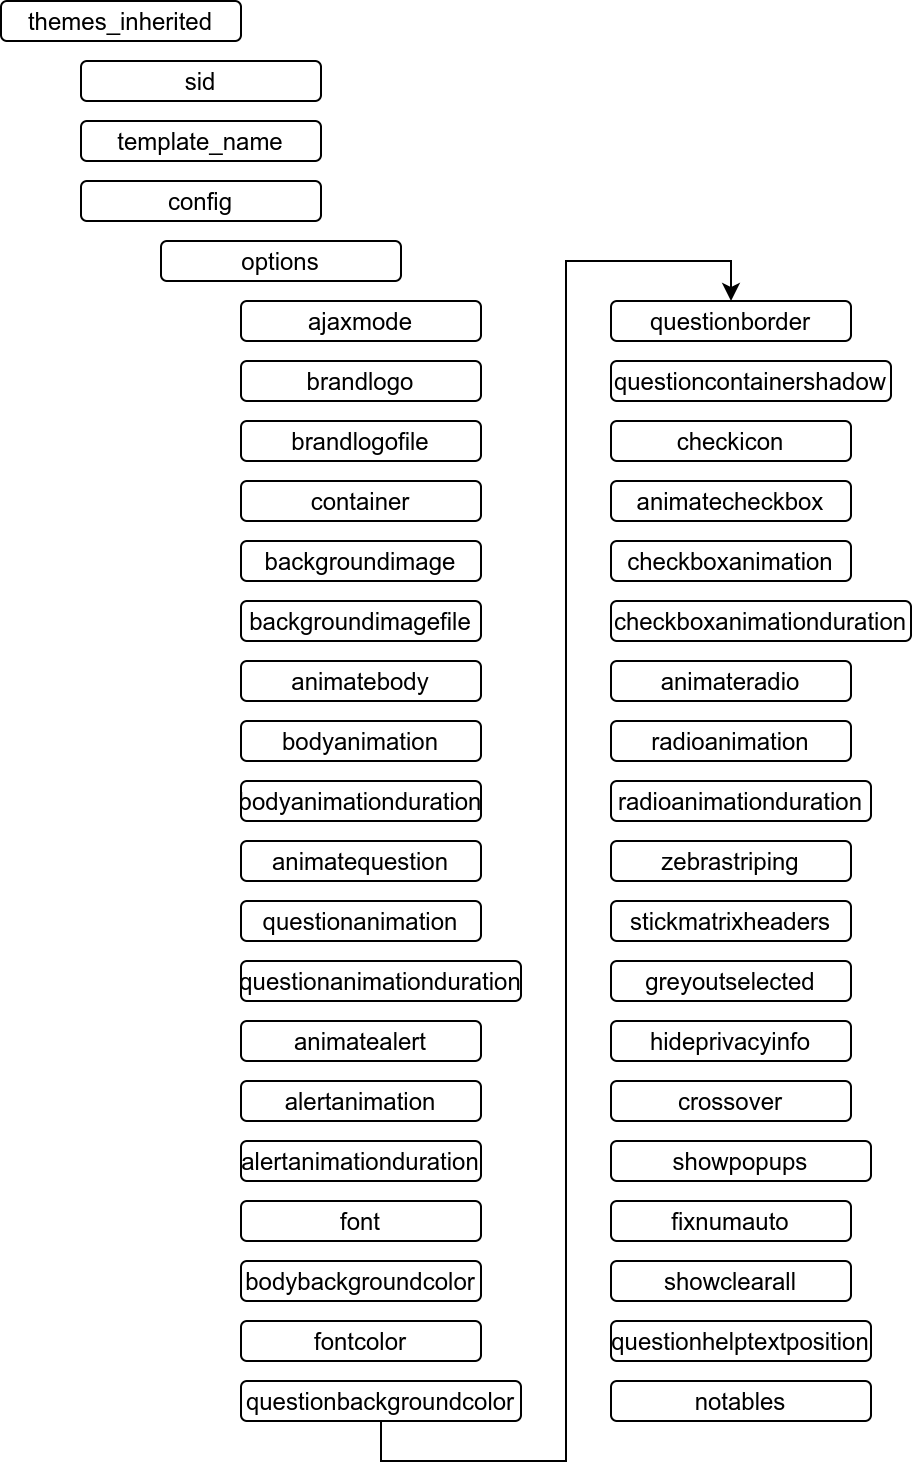
\includegraphics[width=.95\textwidth]{./img/append_lss_theme_inh.png}
	\caption{Aufbau der geerbten Designs}
\end{figure}

\chapter{Klassendiagramme des Programms lsa2odm}

\begin{figure}[h]
	\makebox[\linewidth][c]{%
		\begin{subfigure}[b]{.6\textwidth}
			\label{fig:app}
			\centering
			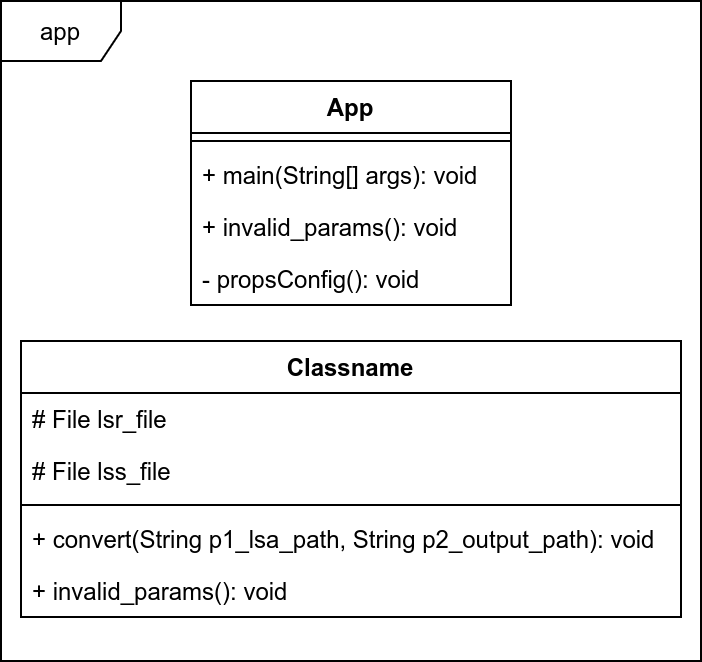
\includegraphics[width=.95\textwidth]{./img/cls_app.png}
			\caption{Klassendiagramm für das Paket \jv{app}}
		\end{subfigure}%
		\begin{subfigure}[b]{.6\textwidth}
			\label{fig:utils}
			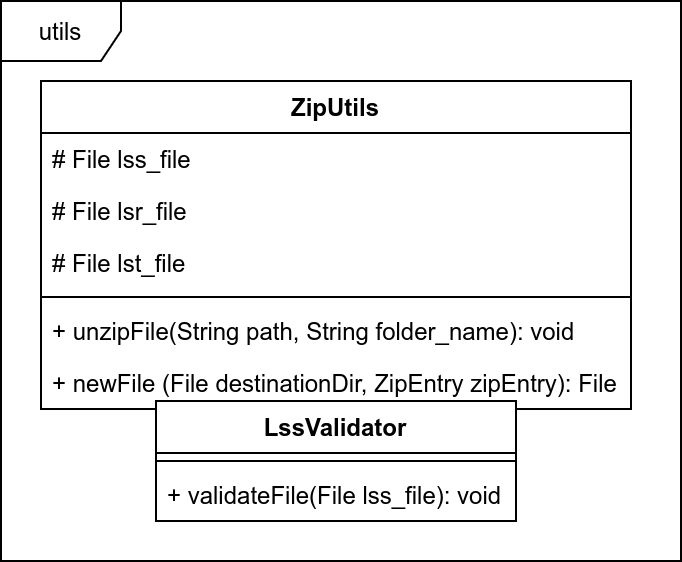
\includegraphics[width=.95\textwidth]{./img/cls_utils.png}
			\caption{Klassendiagramm für das Paket \jv{utils}}
		\end{subfigure}%
		}
		\caption{Klassendiagramme für mehrere Pakete, welche am Anfang der Ausführung gebraucht werden}
\end{figure}

\begin{figure}[h]
	\label{im:fig:lss}
	\centering
	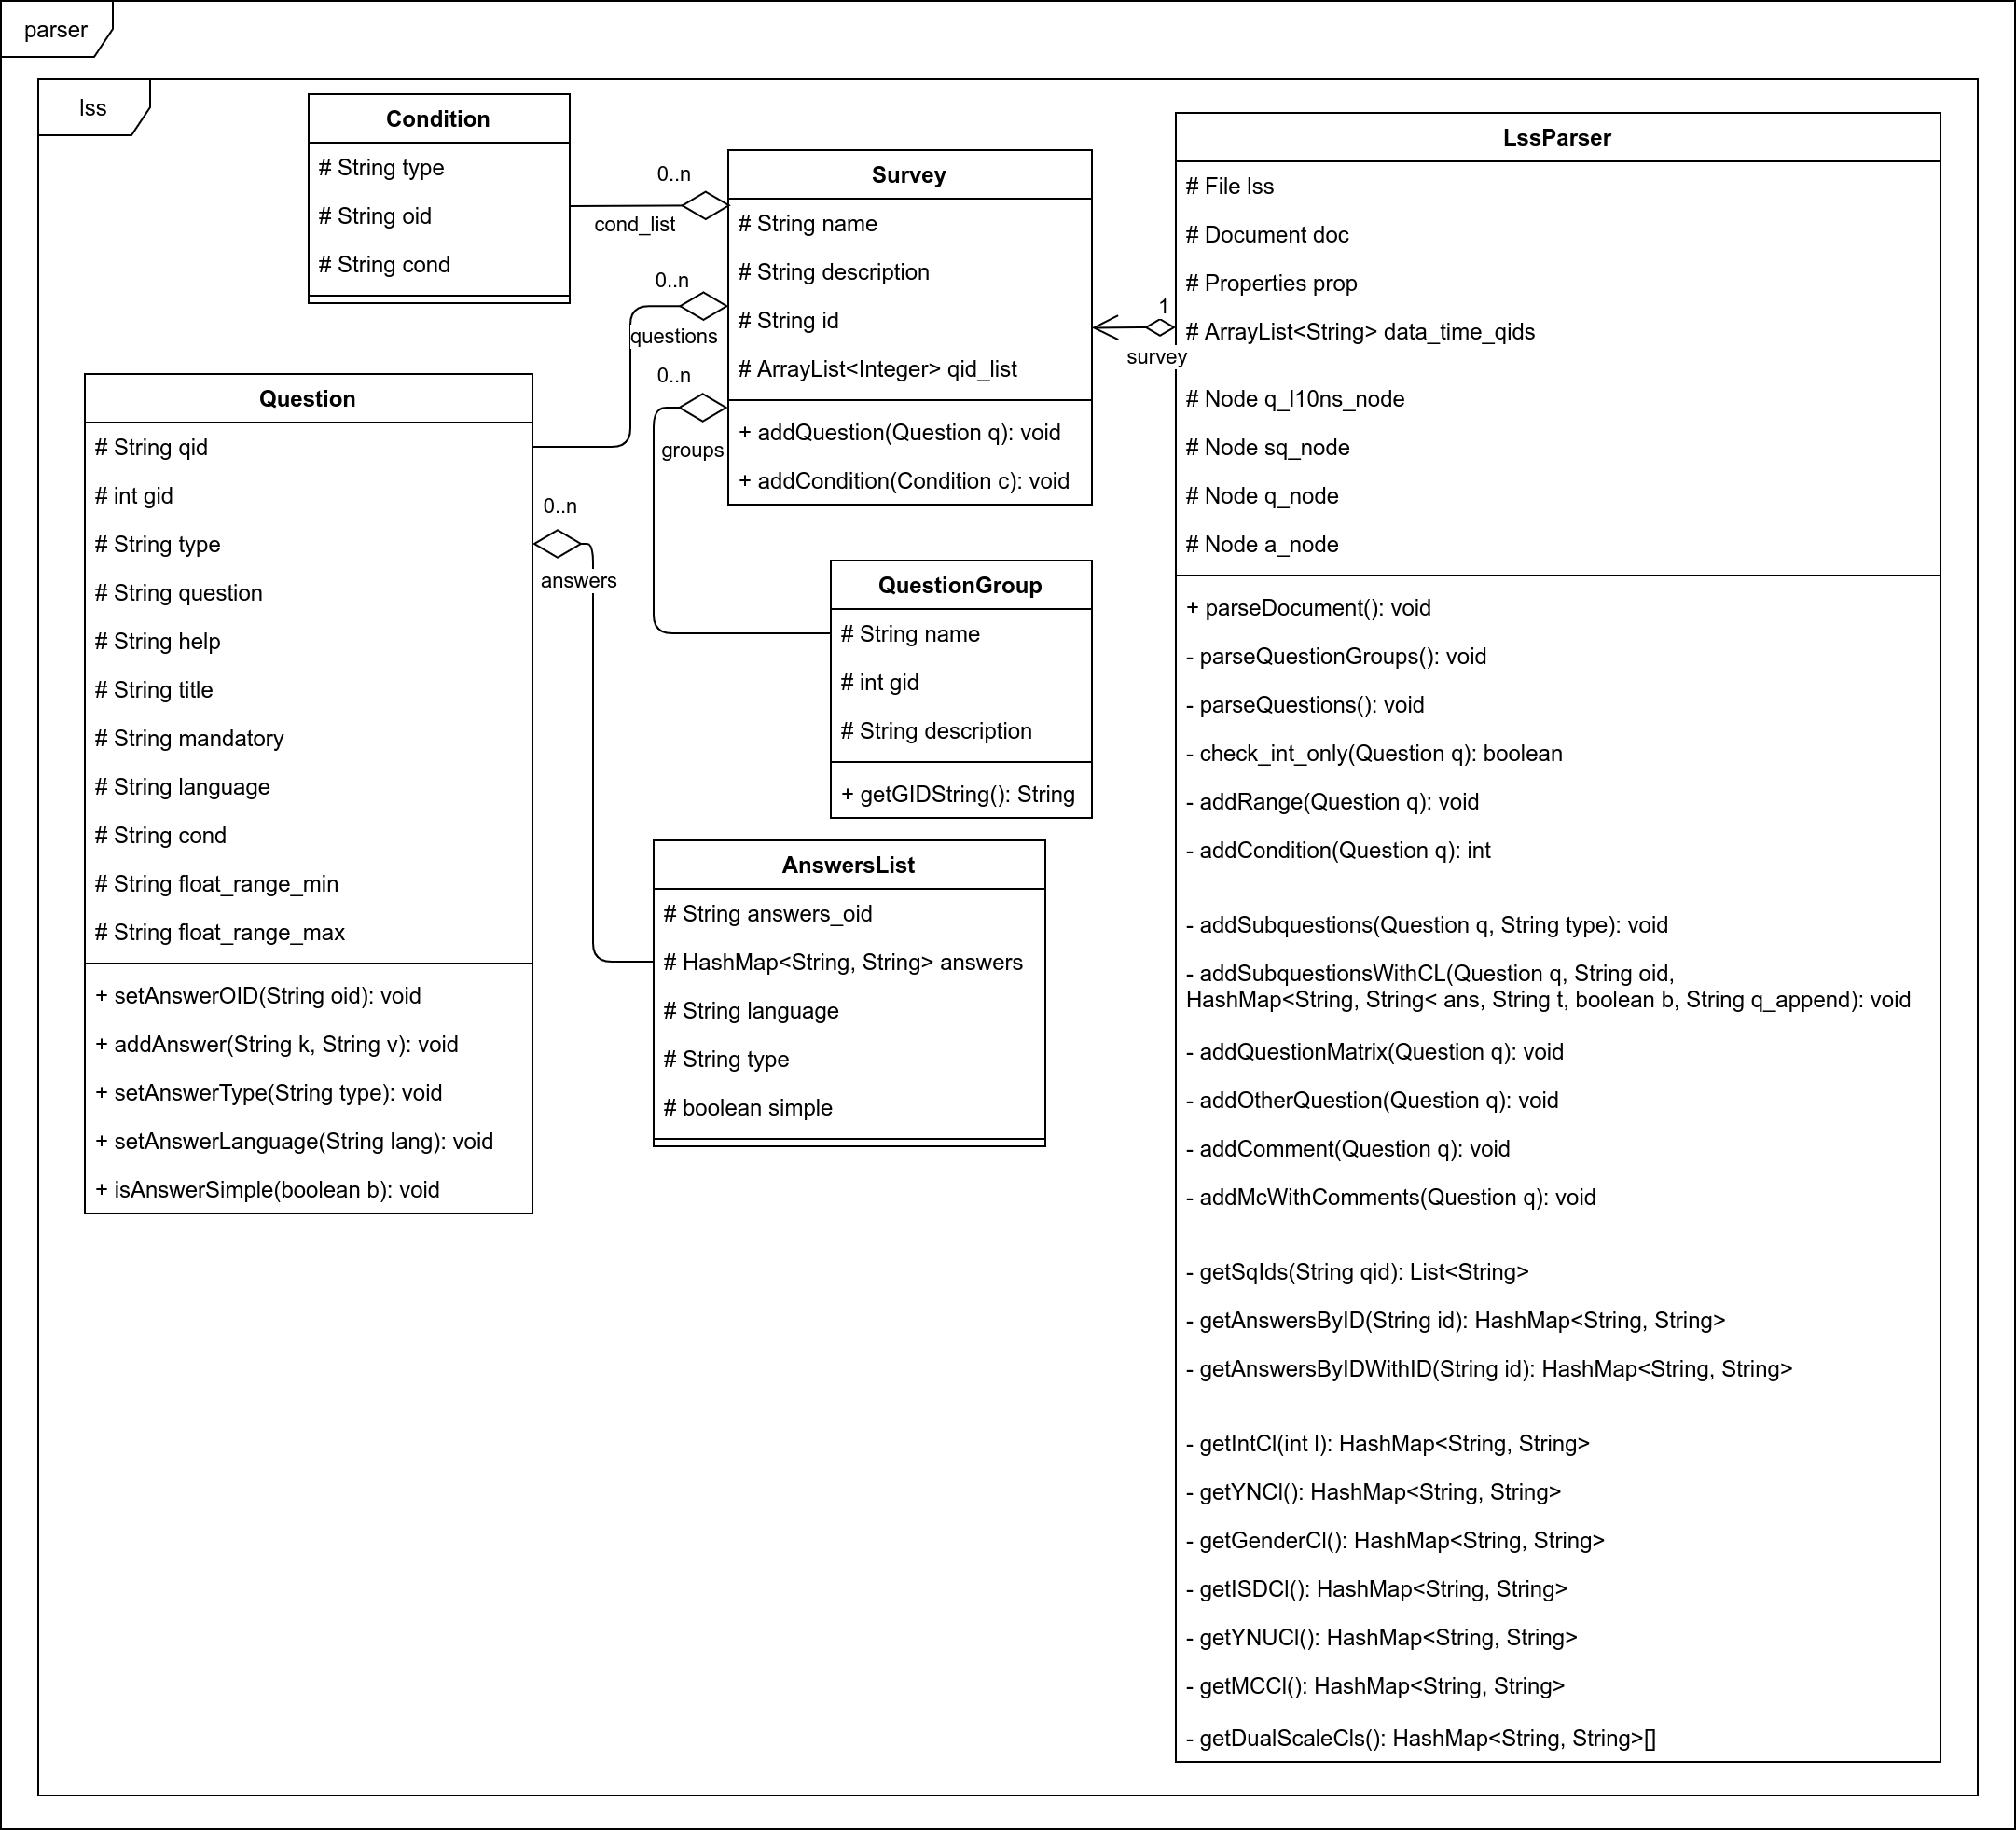
\includegraphics[width=0.90\textwidth]{./img/cls_lss.png}
	\caption{Klassendiagramm für das Paket \textit{lss}}
\end{figure}

\begin{figure}[t]
	\centering
	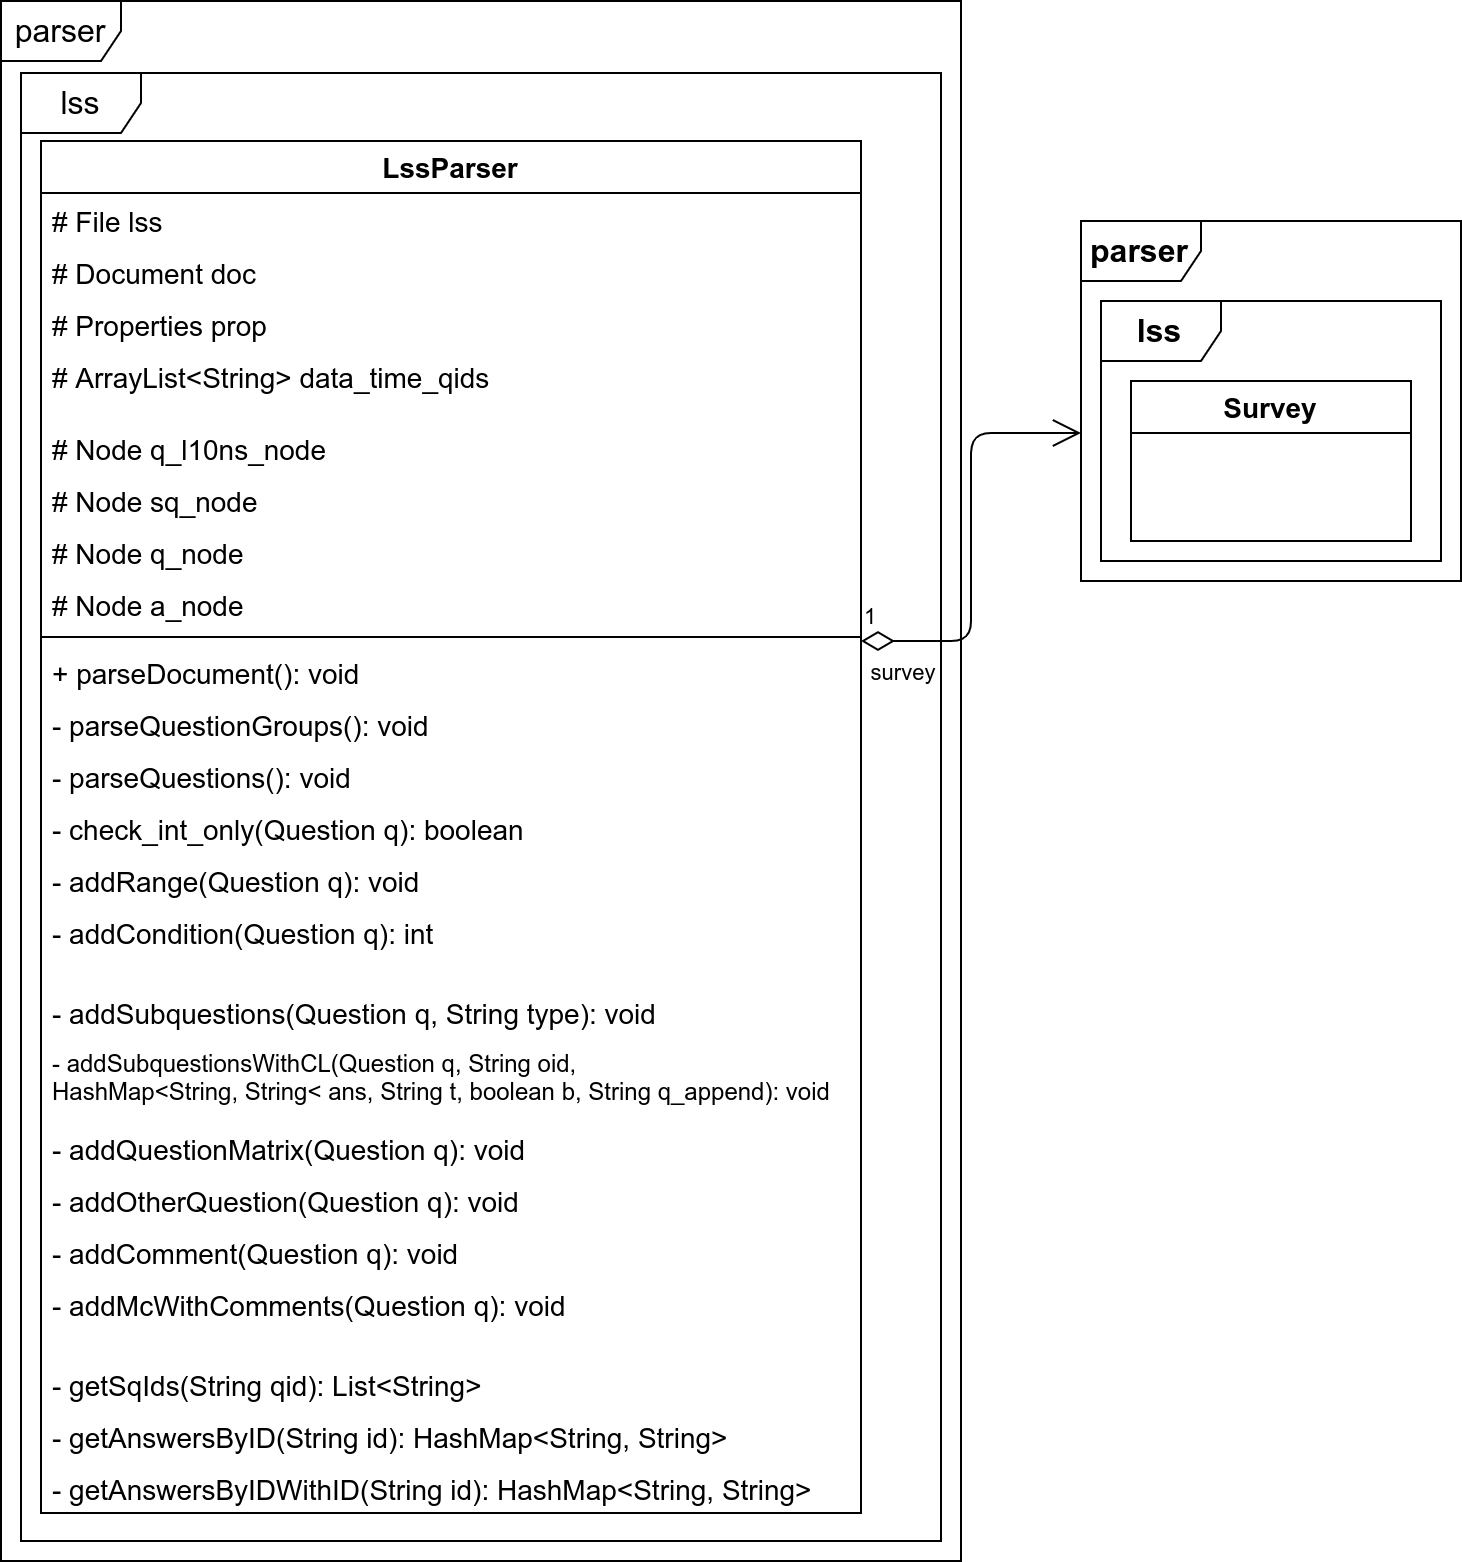
\includegraphics[width=0.99\textwidth]{./img/cls_lss_2.png}
	\caption{Klassendiagramm für \textit{LssParser}}
	\label{fig:lss2}
\end{figure}

\begin{figure}[h]
			\centering
			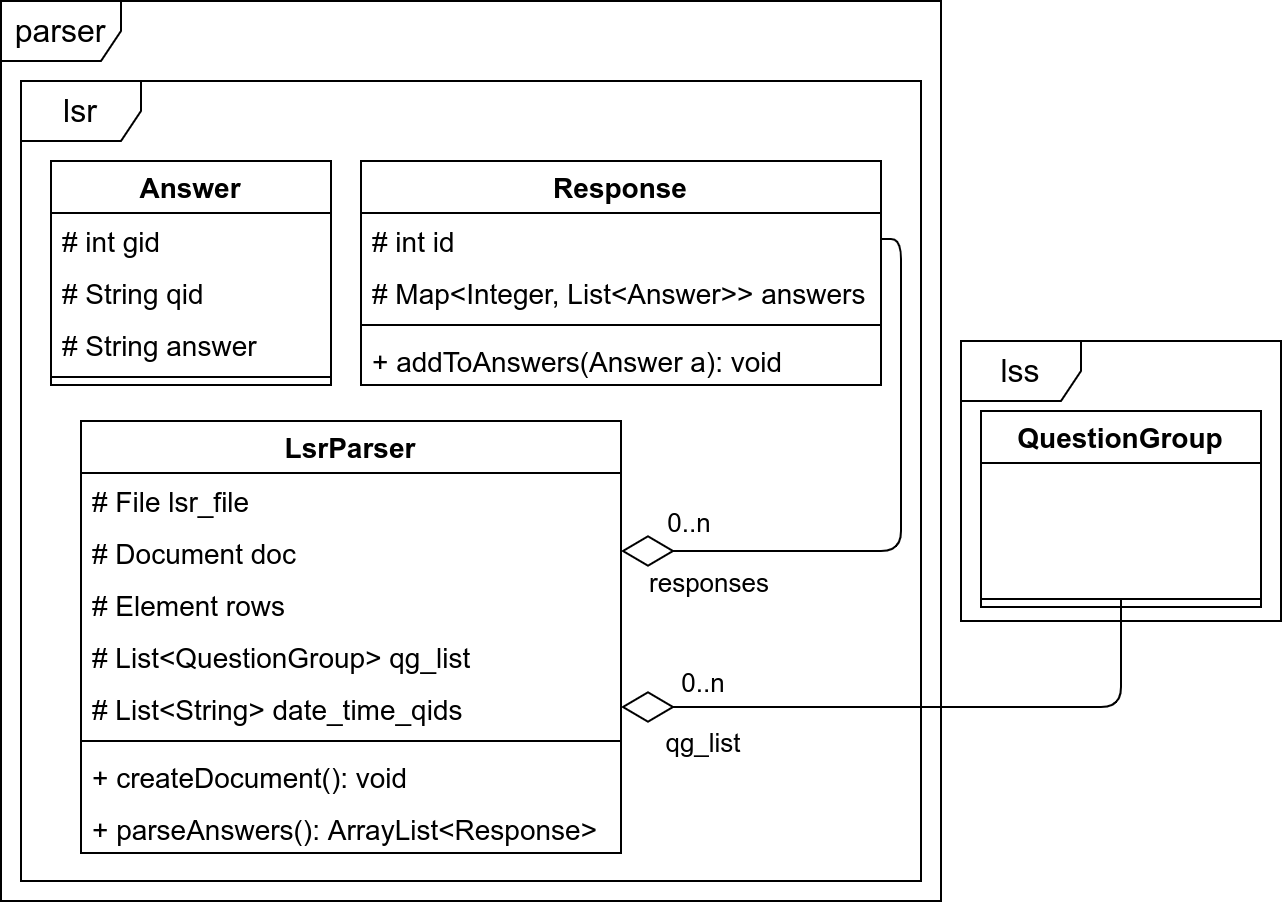
\includegraphics[width=.98\textwidth]{./img/cls_lsr.png}
			\caption{Klassendiagramm des Paketes \textit{lsr}}
\end{figure}

\begin{figure}[h]
	\centering
	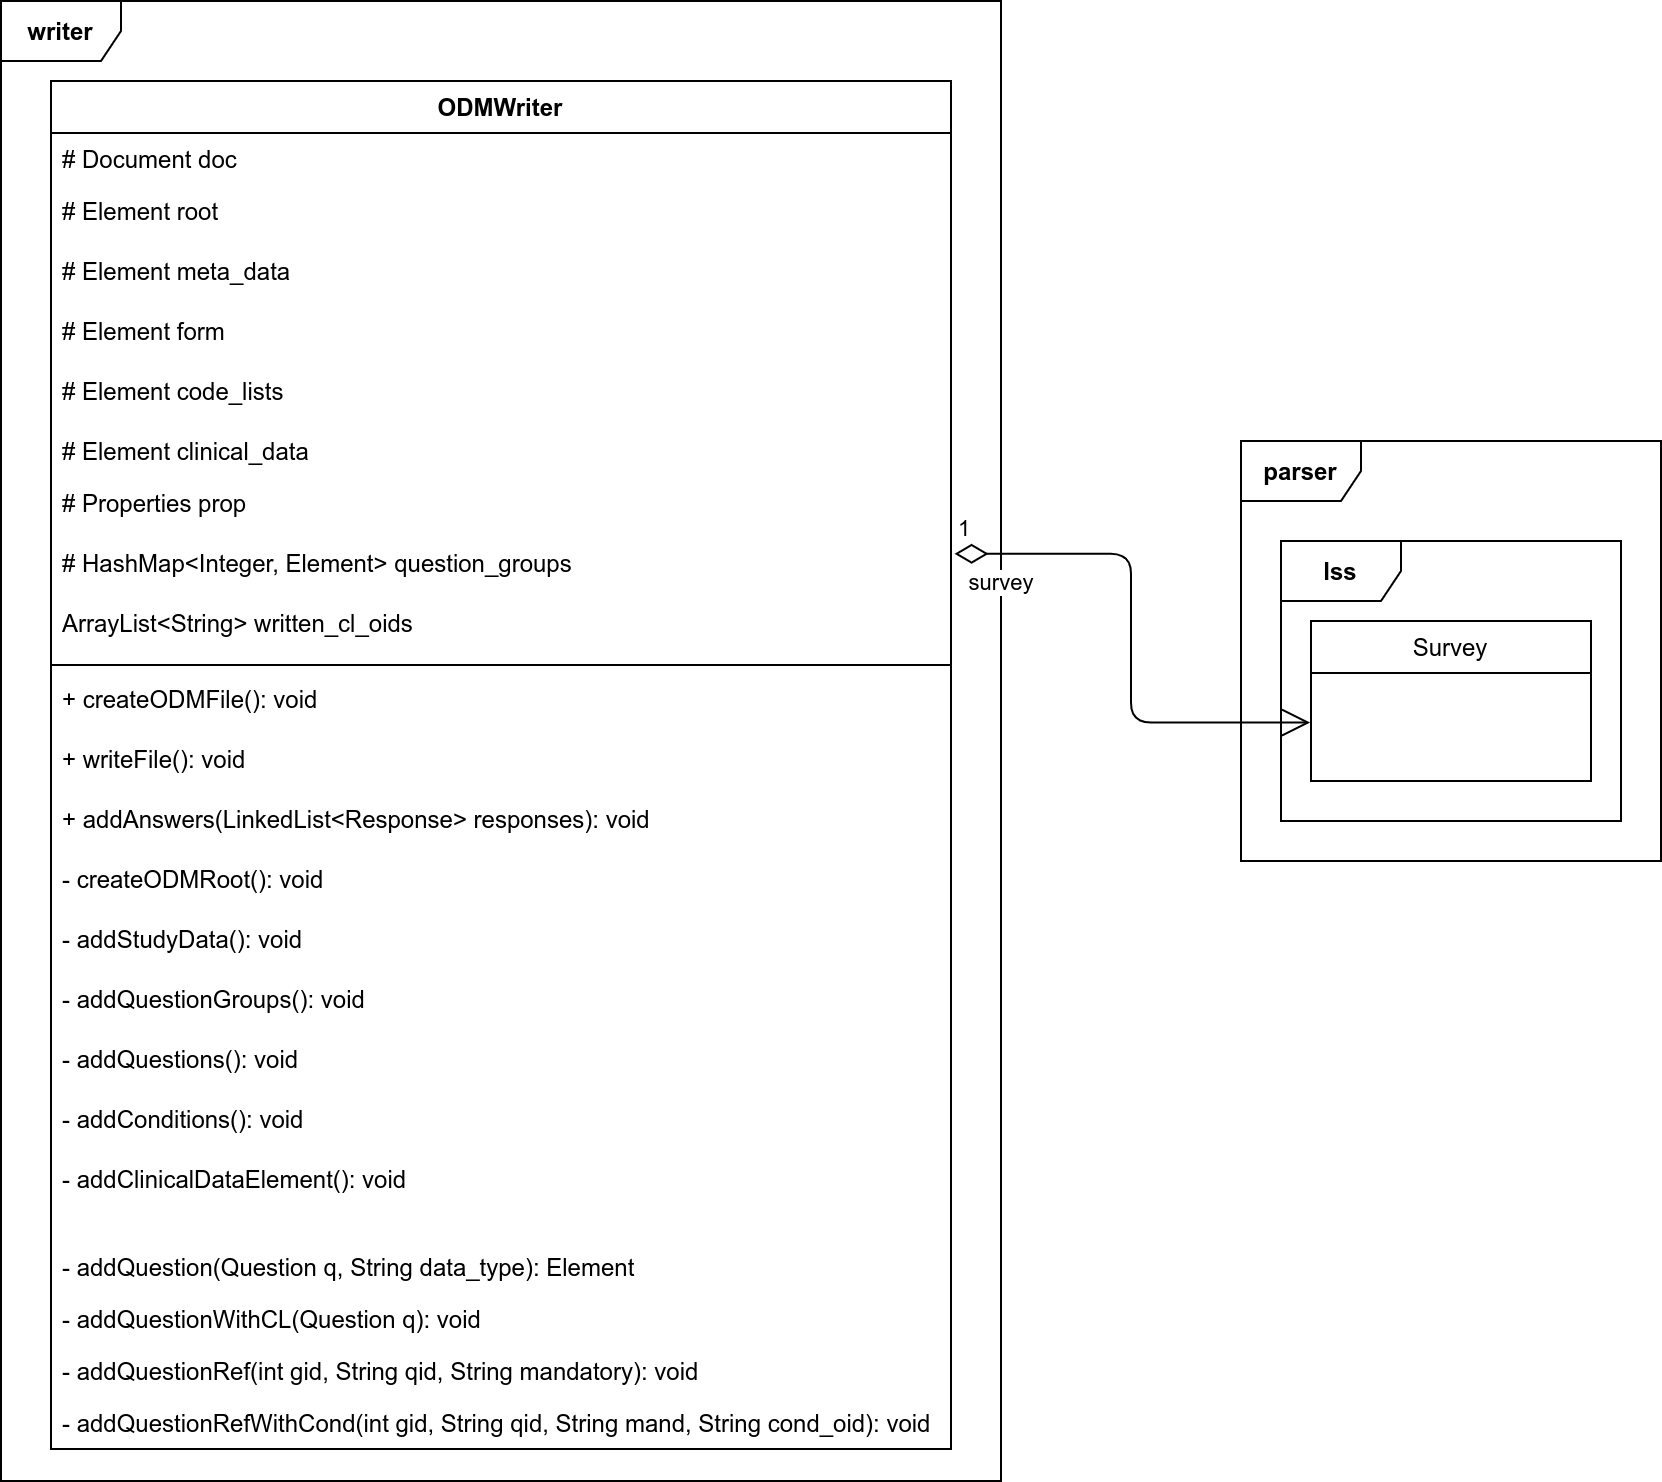
\includegraphics[width=.98\textwidth]{./img/cls_writer.png}
	\caption{Klassendiagramm des Pakets writer}
\end{figure}
